\thispagestyle{empty}
\newgeometry{margin=1in}
\begin{center}

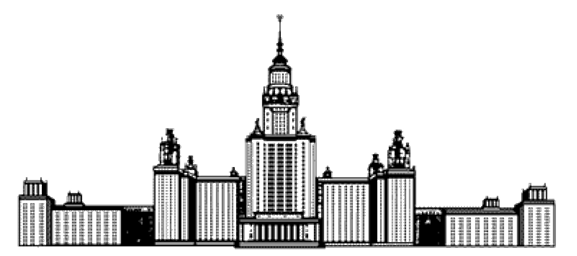
\includegraphics{logo.png}

{
    \large
    Московский государственный университет имени М. В. Ломоносова\par
    Факультет вычислительной математики и кибернетики\par
    Кафедра информационной безопасности\par
}
\par
\end{center}

\vspace{10mm}
\begin{flushright}
%На правах рукописи

{\sl}%УДК xxx.xxx}
\end{flushright}

\begin{center}
%\vspace{10mm}
%{%\small
%Специальность 010200
%
%<<Прикладная математика и информатика>>
%}


\vspace{20mm}
	
\bf \large {Зобов Даниил Сергеевич}

\vspace{5mm}
{
    \bf \large
    Модификация Vorg: автомат с двумя входами и одним выходом и график в единичном кубе 
    
    \par
}
\vspace{5mm}

\textbf{Курсовая работа}

\end{center}

\vspace{40mm}

\begin{flushright}

\textbf{Научный руководитель:}

Профессор, д.ф.-м.н.

Анашин Владимир Сергеевич
\end{flushright}

\vspace{20mm}
\begin{center}
{Москва 2022}
\end{center}

\newpage
